% Todo Goede titel vinden voor Onderzoek Application Security

\chapter{Onderzoek: Application Security}\label{ch:onderzoek:-application-security}

Cyber security wordt steeds belangrijker bij het ontwikkelen van web applicaties.
Met name omdat er een shift gaande is van monolitische applicaties die op personal computers draaien naar (micro) web services die op een server draaien.
De COVID-19 pandemie heeft hier extra in meegeholpen omdat in het bedrijfsleven mensen steeds meer thuis gaan werken en dus ook de applicaties overal beschikbaar moet zijn.
En als we naar het nieuws kijken lijkt het er ook op dat criminelen en spionage diensten hier gretig gebruik van maken door informatie te zoeken om vervolgens te gebruiken tegen een bedrijf of nog erger tegen een natie. Om deze reden is het goed om goed te kijken naar de manieren waarop applicaties beveiligd moeten worden.

Om applicaties te kunnen beschermen tegen vals gebruik moet er vanaf het moment dat er aan ontwikkeld wordt gekeken worden hoe de beveiliging op orde gemaakt moet worden.

Binnen Eaglescience is iedereen zich ervan bewust dat er veilige software gemaakt moet worden. In het onderzoek hiervoor is te lezen wat Eaglescience op het moment van schrijven doet aan preventie en monitoring binnen het ontwikkelen en hosten van een applicatie. Echter, is het goed om eens langs alle mogelijke manier te gaan waarop een applicatie kwetsbaar kan worden. Aan de hand van de OWASP-top10 kan gekeken worden welke zaken er nog missen en waar aangewerkt kan worden.





Dit hoofdstuk beschrijft een literatuur studie die gedaan is om verduidelijking van het onderwerp SOUP en zijn de potentiele gevaren die met zich mee brengen in het gebruik van SOUP. De verduidelijking wordt gegeven in het beantwoorden van een aantal vragen die op komen in de komende onderzoeken.
En zal de lezer helpen met het begrijpen van de zaken die in de komende hoofdstukken worden beschreven.


In het Cybersecuritybeeld Nederland 2020 (CSBN-2020) is te lezen dat de digitale weerbaarheid nog niet overal op orde is.
Wat in feite inhoud dat bedrijven nog niet het vermogen hebben om digitale risico's in voldoende mate te kunnen beheersen.
Dit komt vooral omdat veel systemen( hardware en software) met elkaar verbonden zijn.
En de bijbehorende configuratie niet op orde is.
Een ander feit is dat aanvallers tegenwoordig rondzoeken naar kwetbaarheden in software om zo een mogelijk doelwit te benadelen.
Een goed voorbeeld is het citrix incident op de universiteit van Maastricht eind 2019, waar via een phisingmail toegang werd verleend op servers die vervolgens door lekken software onopgemerkt bleven.
Vervolgens werd er ransomware geplaatst die een groot aantal bestanden versleutelde.
De buit was uiteindelijk € 197.000.

Dit voorbeeld geeft aan dat het niet alleen belangrijk is om de hardware goed te configureren tegen aanvallen.
Maar dat er ook zeker goed gekeken moet worden naar het gebruik van software en hoe deze is opgebouwd.
Software wordt tegenwoordig vaak gebouwd met het gebruik van bibliotheken die SOUP, Software of Unkown Provenance worden genoemd, Contrast Security steld zelfs dat 80\% van de vandaag de dag ontwikkelde software gebruikt maakt van SOUP-bibliotheken.
Waarbij een vierde bekende kwetsbaarheden bevatten.
Het is dus zaak om te onderzoeken of de bibliotheken die gebruikt worden veilig zijn en hier vervolgens desgewenst actie op te nemen als dit nodig is.
%Bron: WhitePaper: The unfortunate reality of insecure Libraries - Contrast security

\section{Wat is Software of Unkown Provenance?}\label{sec:wat-is-soup?}
De term SOUP komt oorspronkelijk de wereld van de ontwikkeling van medische software en staat voor "Software Of Unkown Provenance".
SOUP wordt gezien als een software component dat al ontwikkeld is en beschikbaar is gesteld voor gebruik door een instantie anders dan de gebruiker zonder dat de bewijzen zijn over het bouwen van de software.
Hierdoor is het dus niet duidelijk welk process er is gevolgt tijdens het ontwikkelen en daarmee dus ook de (medische)veiligheid niet is aan te tonen.
De term wordt nu steeds vaker gebruikt in de algemene software ontwikkel kringen om aan te geven dat er van een betreffent software component(framework, bibliotheek, etc.) niet bekend is hoe het ontwikkeld, getest is.
Hierdoor is er dus geen zekerheid dat het component kwetsbaarheden kan bevatten.
Kwetsbaarheden in deze zin zijn dan voornamelijk lekken of veranderingen van functionaliteiten binnen een software.

%Bron: "https://johner-institute.com/articles/software-iec-62304/soup-and-ots/"

\section{Hoe kan het gebruik van SOUP gevaarlijk zijn?}\label{sec:hoe-kan-het-gebruik-van-soup-gevaarlijk-zijn?}
Uit een onderzoek van Contrast Security blijkt dat 80\% van de broncode die vandaag de dag gebruikt wordt om een applicatie te schrijven bestaat uit broncode uit een externe bibliotheek.
Waarbij een vierde van de gedownloade bibliotheken kwetsbaarheden bevatten.
De kans dat er dus onbekende kwetsbaarheden in een applicatie sluipen is dus zeker aanwezig.
Een van de redenen dat dit kan gebeuren is een fenomeen dat een package dependency network wordt genoemd.
Wat in het kort betekend dat een dependency die je als ontwikkelaar gebruikt zelf ook een aantal dependencies heeft, welke op zijn beurt ook weer dependecies heeft.
[verder uitwerken]
Dit kan in theorie vele lagen bevatten waardoor de structuur minder inzichtelijk wordt omdat er voor iedere dependency in het netwerk een assesment gedaan moet worden naar kwetsbaarheden.
In verschillende artikelen(Bronnen) wordt gewaarschuwd voor het gevaar van het gebruik deze constructie, echter lijkt het erop dat er binnenkort niet echt verandering komt in de manier waarop dependencies worden gelinkt.
Een andere oplossing zou dan zijn om iedere depenency te checken op kwetsbaarheden tegen een database
Bron: On the inpact of security vulnerabilities in npm package dependency network - Alexandre Decan, Tom Mens, Eleni Constantinou (2018), Structure and Evolution of package dependency networks.

\section{Instanties en SOUP}\label{sec:instanties-en-soup}
Kwetsbaarheden binnen softwareontwikkeling is niet iets van de laatste tijd en er zijn gelukkig instanties die zich bezig houden met het veilighouden van software door middel van trainingen, lezingen en andere manieren van awareness opwekken.
Sommige instanties houden bij welke kwetsbaarheden er gevonden zijn en plaatsen dit in een CVE-database.
Anderen melden veel voorkomende kwetsbaarhden in een top-10

\subsection{CVE Databases, MITRE, NIST, NVD}\label{subsec:mitre-nist-nvd}
CVE staat voor Common Vulenerabilities en Exposures wat een database waarin kwetsbaarheden staan die gevonden zijn in de verschillende systemen.
Deze Database wordt voornamelijk bijgehouden door het bedrijf MITRE dat met subsidie van de US Division of Homeland Security werkt aan het kenbaar maken van lekken in software\footnote{Software wordt hier gezien in de ruimste zin van het woord hierbij hoort: Operating systems, open en closed source software. maar ook frameworks en bibliotheken.}.
De CVE's die in deze database staan worden vervolgens geannalyseerd door het NIST(National Institute os Standards and Technology) en voorzien van een CVSS\footnote{Common Vulnerability Score System is een gestandardiseerde manier om een score aan een kwetsbaarheid toe te kennen waarop in een enkel oog opslag te zien is hoe rieel een risico is.} score en geplaats in de NVD-database.
Zowel de database van MITRE (https://cve.mitre.org) als NIST (https://nvd.nist.gov) zijn publiekelijk toegankelijk.

\subsection{OWASP}\label{subsec:owasp}
Naast het bijhouden van CVE's in database is het creëren van awareness net zo belangrijk.
Een instantie die zich bezig houd hier mee is OWASP(Open Web Application Security Project) die awareness creëert door ideree 5 jaar\footnote{helaas is op het moment van schrijven de laatste versie(2021) nog niet uitgebracht en staat hier de versie uit 2017} een Top-10 uit te brengen met daarin de meest voorkomende en dreigende kwetsbaarheden die ze gevonden hebben in een dataset wat opgebouwd is uit inzendingen van 500+ onderzoekers van 40+ bedrijven die samen meer dan 100.000 API's en web applicaties hebben onderzocht.
In de top 10 die hieronder samengevat weer wordt gegeven wordt er een score meegegeven over hoe makkelijk een lek is te ontdekken en welk mate van risico de kwetsbaarheid heeft.

\begin{figure}[H]
    \myfloatalign
    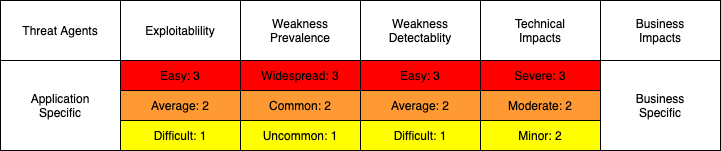
\includegraphics[width=12cm]{gfx/risk tabel}
    \caption{Inschaling van risico's door OWASP}
    \label{fig:risico inschaling}
\end{figure}

\begin{itemize}
%Bron: https://codebros.nl/blog/wat-is-de-owasp-top-10 , https://owasp.org/www-project-top-ten/ << PDF download

    \item \textbf{A01:2017 Injection[exploitabity: 3, Prevelance: 2, detectability: 3, technical: 3]:}

    De mogelijkheid om OS, SQL, NoSQL commandos te injecteren in web applicaties zorgt ervoor dat aanvallers toegang kunnen hebben tot delen van systemen zonder er recht op te hebben.
    Daarnaast is er ook de mogelijkheid om toegang te krijgen tot data die niet voor hen bedoelt is.


    \item \textbf{A02:2017 Broken Authentication[exploitabity: 3, Prevelance: 2, detectability: 2, technical: 3]:}

    Het verkeerd implementeren van authentication en session management kan er voor zorgen dat aanvallers wachtwoorden, sessie tokens aan kunnen passen om zo zich voor te doen als een andere gebruiker.

    \item \textbf{A03:2017 Sensitive Data Exposure[exploitabity: 2, Prevelance: 3, detectability: 2, technical: 3]:}

    Het verkeerd of niet voldoende afschermen van API's kunnen ervoor zorgen dat sensitive data makkelijk gevonden kan worden.\ Zeker als de data niet encrypted verzonden wordt.

    \item \textbf{A04:2017 XML External Entities (XXE)[exploitabity: 2, Prevelance: 2, detectability: 3, technical: 3]:}

    Veel oude of slecht geconfigureerde XML-processoren evalueren externe entiteit referenties binnen XML-documenten slecht.\ Hierdoor is het mogelijk om links te creeën naar bestanden en/of fileshares waar code staat die slecht is voor de applicatie [that contains malicious code].

    \item \textbf{A05:2017 Broken Access Control[exploitabity: 2, Prevelance: 2, detectability: 2, technical: 3]:}

    Beperkingen op wat een geauthenticeerde gebruikers mogen worden niet altijd nageleefd, Aanvallers kunnend deze fouten gebruiken om toegang te krijgen tot gegevens of functionaliteiten die niet bestemd zijn voor deze gebruikers.\ Ze kunnen gegevens aanpassen en / of toegangsrechten aanpassen.

    \item \textbf{A06:2017 Security Misconfiguration[exploitabity: 3, Prevelance: 3, detectability: 3, technical: 2]:}

    Slechte configuratie van de veiligheids instellingen zijn de meest gevonden probleem.\ Dit is meestal het gevolg van het gebruiken van de default, incomplete of ad hoc configuratie Hierdoor kunnen cloud storages open komen te staan, verkeerd geconfigureerde HTTP-headers of foutmeldingen die te veel informatie meegeven ontstaan.

    \item \textbf{A07:2017 Cross-Site Scripting (XSS)[exploitabity: 3, Prevelance: 3, detectability: 3, technical: 2]:}

    Middels XSS is het mogelijk om scripts te draaien van een andere bron dan wenselijk.\ Dit geeft de mogelijkheid om via een browser andere scripts in de applicatie te draaien zo proberen andere functionaliteiten toe te voegen.\ Wat kan leiden tot een web-site dat zich anders gedraagt dan de bedoeling is.

    \item \textbf{A08:2017 Insecure Deserialization[exploitabity: 1, Prevelance: 2, detectability: 2, technical: 3]:}

    Door het niet veilig serialiseren van objecten naar text kan het voorkomen dat er code of commando's mee worden gestuurd welke uitgevoers kunnen worden op de server.

    \item \textbf{A09:2017 Using components with Known vulnerabilities[exploitabity: 2, Prevelance: 3, detectability: 2, technical: 2]:}

    Componenten zoals bibliotheken, frameworks en andere software modules die gebruikt worden voor het ontwikkelen van een applicatie kunnen bedoeld of onbedoeld kwaadaardige code bevatten Wat kan leiden tot verschillende mogelijkheden voor de aanvaller binnen te dringen.\ Of data te versturen naar een andere host om zo achter "beveiligde" gegevens te komen.

    \item \textbf{A10:2017 Insuffivient Logging \& Monitoring[exploitabity: 2, Prevelance: 3, detectability: 1, technical: 2]:}

    Logging en monitoring is bijna net zo belangrijk als het ontwikkelen van een veilige applicatie, mocht er toch een aanval plaatsvinden op welke manier dient er de mogelijkheid zijn om terug te zien wat er precies gebeurt is.\ Logging zorgt hiervoor.\ Het monitoring deel is het bekijken van de logs om te zien of er iets verdachts plaats heeft gevonden.\ Er zijn tools beschikbaar die er voor automatische monitoring zorgen( Nagios is dit soort tool)

\end{itemize}

%Bronnen:
%https://www.imperva.com/learn/application-security/cve-cvss-vulnerability/
%http://owasp.org
\section{Invloed van SOUP op veiligheid van software}\label{sec:invloed-van-soup-op-veiligheid-van-software}
In de OWASP top-10 staat op plaats 9 "Using components with known vulnerabilities" wat aangeeft dat het op het moment van schrijven aandacht nodig heeft.
Eén van de redenen dat dit probleem in de top 10 staat is omdat het gebruik van bibliotheken bijna niet te vermijden is in de ontwikkeling van applicaties wat vooral te danken is aan het steeds sneller moet leveren van een product.
Ontwikkelaars zijn nooit volledig op de hoogte van de werking laat staan wie de onwikkelaar is van een externe bibliotheek.
Een goed voorbeeld hiervan is de "event-stream vulnerability" waarbij de bibliotheek voorzien werd van crypto-coin-stealing malware.
Dit kon gebeuren omdat de bibliotheek niet meer actief werd onderhouden en een persoon zich aanmelde om de ontwikkeling over te nemen.
Vervolgens werd een dependency omgezet van versie en functionaliteit waardoor er toegang werd, verleent om crypto coins te stelen.
Event-stream is een bibliotheek dat veel gebruikt werd als dependency voor applicaties de stream-functionaliteiten van nodejs gebruikten daardoor heeft het de potentie gehad om veel schade aan te richten.
Het is niet geheel duidelijk hoeveel schade er is gelden echter laat dit voorbeeld duidelijk zien wat het probleem is en hoe snel je kan verdwalen in dependency tree's.
Een oplossing is om regelmatig te scannen naar verdachte bibliotheken in de dependency tree.
En er vervolgens actief mee om te gaan door bibliotheken up-to-date te houden.
%Bron: https://www.theregister.com/2018/11/26/npm_repo_bitcoin_stealer/

\section{Dependency trees?}\label{sec:dependency-trees?}
Een dependency tree is een boom structuur waarin staat welke bibliotheken er gebruikt worden door een applicatie en kan beschikken over meerdere lagen.
Laten we als voorbeeld het boven genoemde "event-stream" npm package nemen.
Op de npm website staat vermeld dat deze package ondersteuning biedt aan 1895 andere pakketten en zelf 7 dependencies heeft.
Nu moet je als je zeker wil weten of er kwaadwillende broncode deze ook scannen. 
Als we kijken hoeveel dependencies deze weer hebben komen op 4 depenendies die ieders weer dependencies hebben.
De tree van Event-stream is hier te vinden, de kwaadaardige package waar het mis mee ging is verwijderd uit de dependency tree door waarschijnlijk een andere oplossing te vinden.

\begin{figure}[H]
    \myfloatalign
    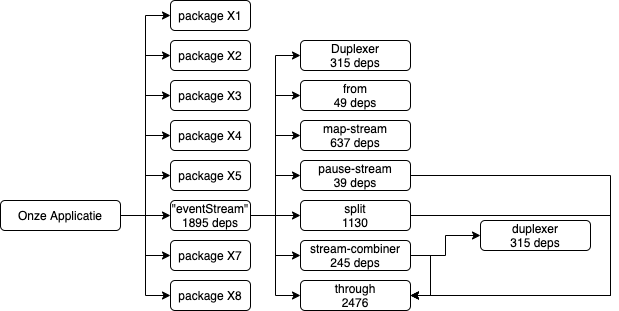
\includegraphics[width=12cm]{gfx/dependency-tree}
    \caption{Dependency tree}\label{fig:dependency-tree}
\end{figure}
Een applicatie heeft niet één zo'n boom maar voor iedere package in de eerste kolom bestaat zo'n boom die dus nog dieper kan gaan dan de hier afgebeelde.
Handmatig scannen is dus geen optie.
Dus moet de oplossing gezocht worden in het autmatisch scannen, gelukkig bestaan er een aantal scanners voor NPM depencies, zxoals versions en retire.js.
Maar ook voor Java en .NET bestaat er een dependency checker ontwikkeld door de OWASP\@.


